%=== CHAPTER FIVE (5) ===
%=== Discussion ===

\chapter{Discussion}

\section{Results of multi ground robots cluster}
\label{sec:disussmultiground}

Seen graphically according to Figure \ref{fig:kittiresults}, the mapping results of CORB-SLAM clients is able to match the ground truth trajectory fairly well enough. And seeing the numeric analysis in Table \ref{tbl:kittiquanresult}, the completed map fused by the server has $8.34\%$ mean relative translation error and $0.54^\circ$ mean relative yaw error with all distance traveled.

Comparing the fused map with the mapping results on the original unseparated sequence, according to the differences between Table \ref{tbl:kittiquanresult} and \ref{tbl:kitticlientquanresult}, map fusion in CORB-SLAM server slight reduces the accuracy on relative yaw and scaling. However from the table, the relative translation accuracy is numerically increased, of which a critical reason is the distance traveled by each client is inevitable shortened because the sequence is divided into two parts, which means translation errors on each client are accumulated during shorter distances. Therefore, it is not concluded so far that map fusion module in server can increase accuracy of relative translation.

Evaluation on KITTI Dataset is an ideal circumstance, with all overlapped images identical. To evaluate under a more general real-world circumstance to get more universal and convincing results, another evaluation is performed utilizing NTU Dataset. 

According to the comparison of quantitative map fusion result ( in Figure \ref{fig:ntuquanresult} and Table \ref{tbl:ntuquanresult} ) and mapping results of single bags ( in Figure \ref{fig:ntubag0quanresult}, \ref{fig:ntubag1quanresult} and Table \ref{tbl:ntubag0quanresult}, \ref{tbl:ntubag1quanresult} ), compared to 6.32$\%$ relative translation error of client of Bag.0, and 30.70$\%$ of Bag.1, the global fused map in server has an error of 23.77$\%$, which can be considered as an acceptable result, considering Bag.1 has a complicated trajectory consisting both parts of indoor and outdoor environment causing client map has a relatively higher translation error.

%\section{Results of multi hybrid robots cluster}
%\label{sec:disussmultihybrid}

\section{Failure Reasons and Drawbacks of Illumination Variance Method}
\label{sec:discusslifelong}

According to the ground truth information of the selected partial sequences of Oxford RobotCar Datasets, the correct fused estimate trajectories of clients should be coincident with very little offset seen as Figure \ref{fig:robotcarseq01servergt}. However as shown in Figure \ref{fig:robotcarmfresult}, integrating CORB-SLAM system with illumination variance failed to enhance the ability to deal with illumination and season changes in Oxford RobotCar Datasets. 

As seen in Figure \ref{fig:robotcarmfresult}, illumination variance method introduce many incorrect matches of keypoints while it is expected to allow ORB matcher to find more correct keypoint pairs that hard to match in raw images due to illumination changes. 

By analyzing the basic formula to compute illumination variance, Equation \ref{eq:iifinal} which is repeated below as Equation \ref{eq:discussiifinal} for reference, and the result images in Figure \ref{fig:discussrobotcarill}, the following reasons and drawbacks of illumination variance method can be concluded to explain the failure of it to help CORB-SLAM deal with images under different illumination conditions and seasons: 

\begin{equation}
I=\log(G)-\alpha\log(B)-(1-\alpha)\log(R)
\label{eq:discussiifinal}
\end{equation}

\begin{enumerate}[1.]
	\item Loss of resolution. According to the computation shown in Equation \ref{eq:discussiifinal}, there are two steps in this method to calculate the value of illumination variance: for each pixel, 
		\begin{inparaenum}[1)]
			\item logarithm of r,g, b channel values,
			\item take their weighted difference as the result illumination variance value.
		\end{inparaenum}
	Both steps cause serious loss of resolution, with the result image very blurry as seen in Figure \ref{fig:discussrobotcarill}. 
	
	\item Requirement of high brightness and contrast of input color images. In Figure \ref{fig:discussrobotcarill}, compared to Figure \ref{sfig:robotcarjulyill}, Figure \ref{sfig:robotcarjulyill} has a higher resolution. This is because with the loss of resolution during the illumination variance computation, images with higher brightness and contrast can remain more details in the result images. But the background of application of this method is in life-long localization and mapping system, running under significant lighting and season conditions, which means it is an unreasonable request to demand the input images always bright and sharp.
	
%	\item Because of loss of resolution, obviously the position information of keypoints in illumination variance images are not accurate enough to estimate trajectories within acceptable errors. To solve this problem, the initial idea in this work is when close loops are detected in illumination variance images, the visual odometer module 
\end{enumerate}


\begin{figure}
	\centering
	\subfigure[Corresponding illumination variance image of Figure \ref{sfig:robotcarjulyraw}.]{
		\begin{minipage}[t]{\linewidth}
			\label{sfig:robotcarjulyill}
			\centering
			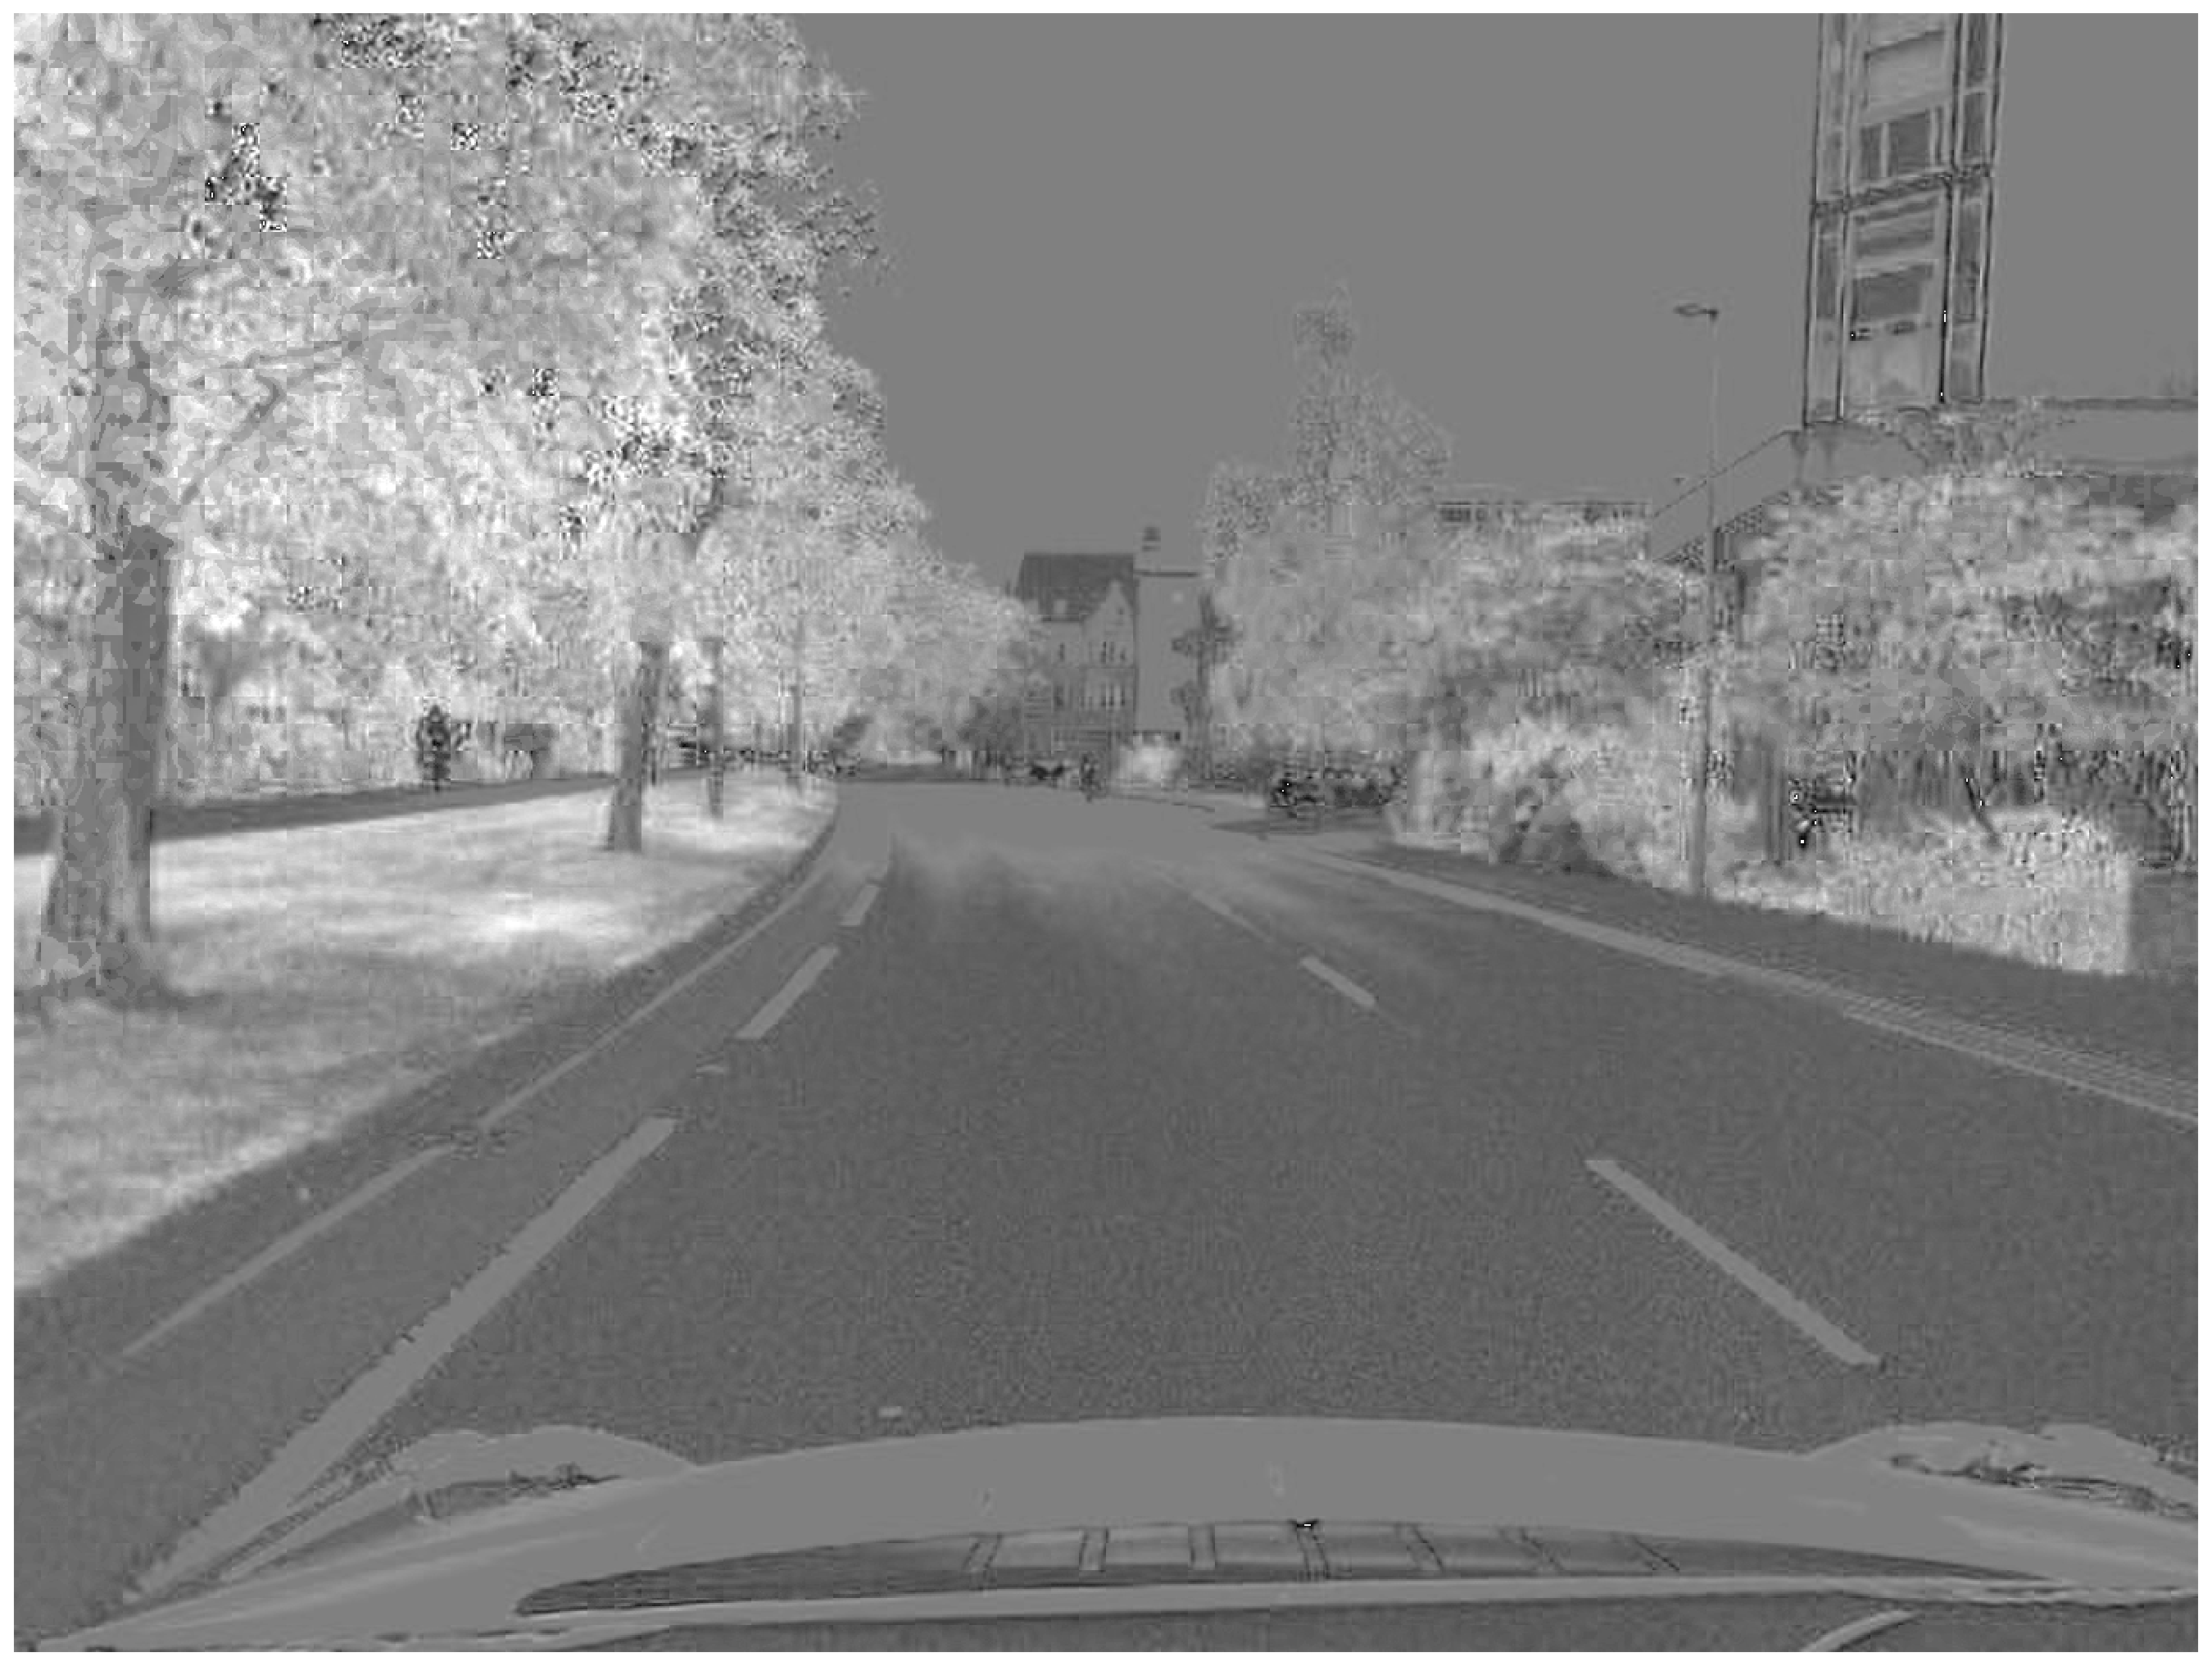
\includegraphics[width=4in]{Chapter4/robotcar/ill_inv1.eps}
			%\caption{fig1}
		\end{minipage}
	}
\vfill
	\subfigure[Corresponding illumination variance image of Figure \ref{sfig:robotcarfebraw}.]{
		\begin{minipage}[t]{\linewidth}
			\label{sfig:robotcarfebill}
			\centering
			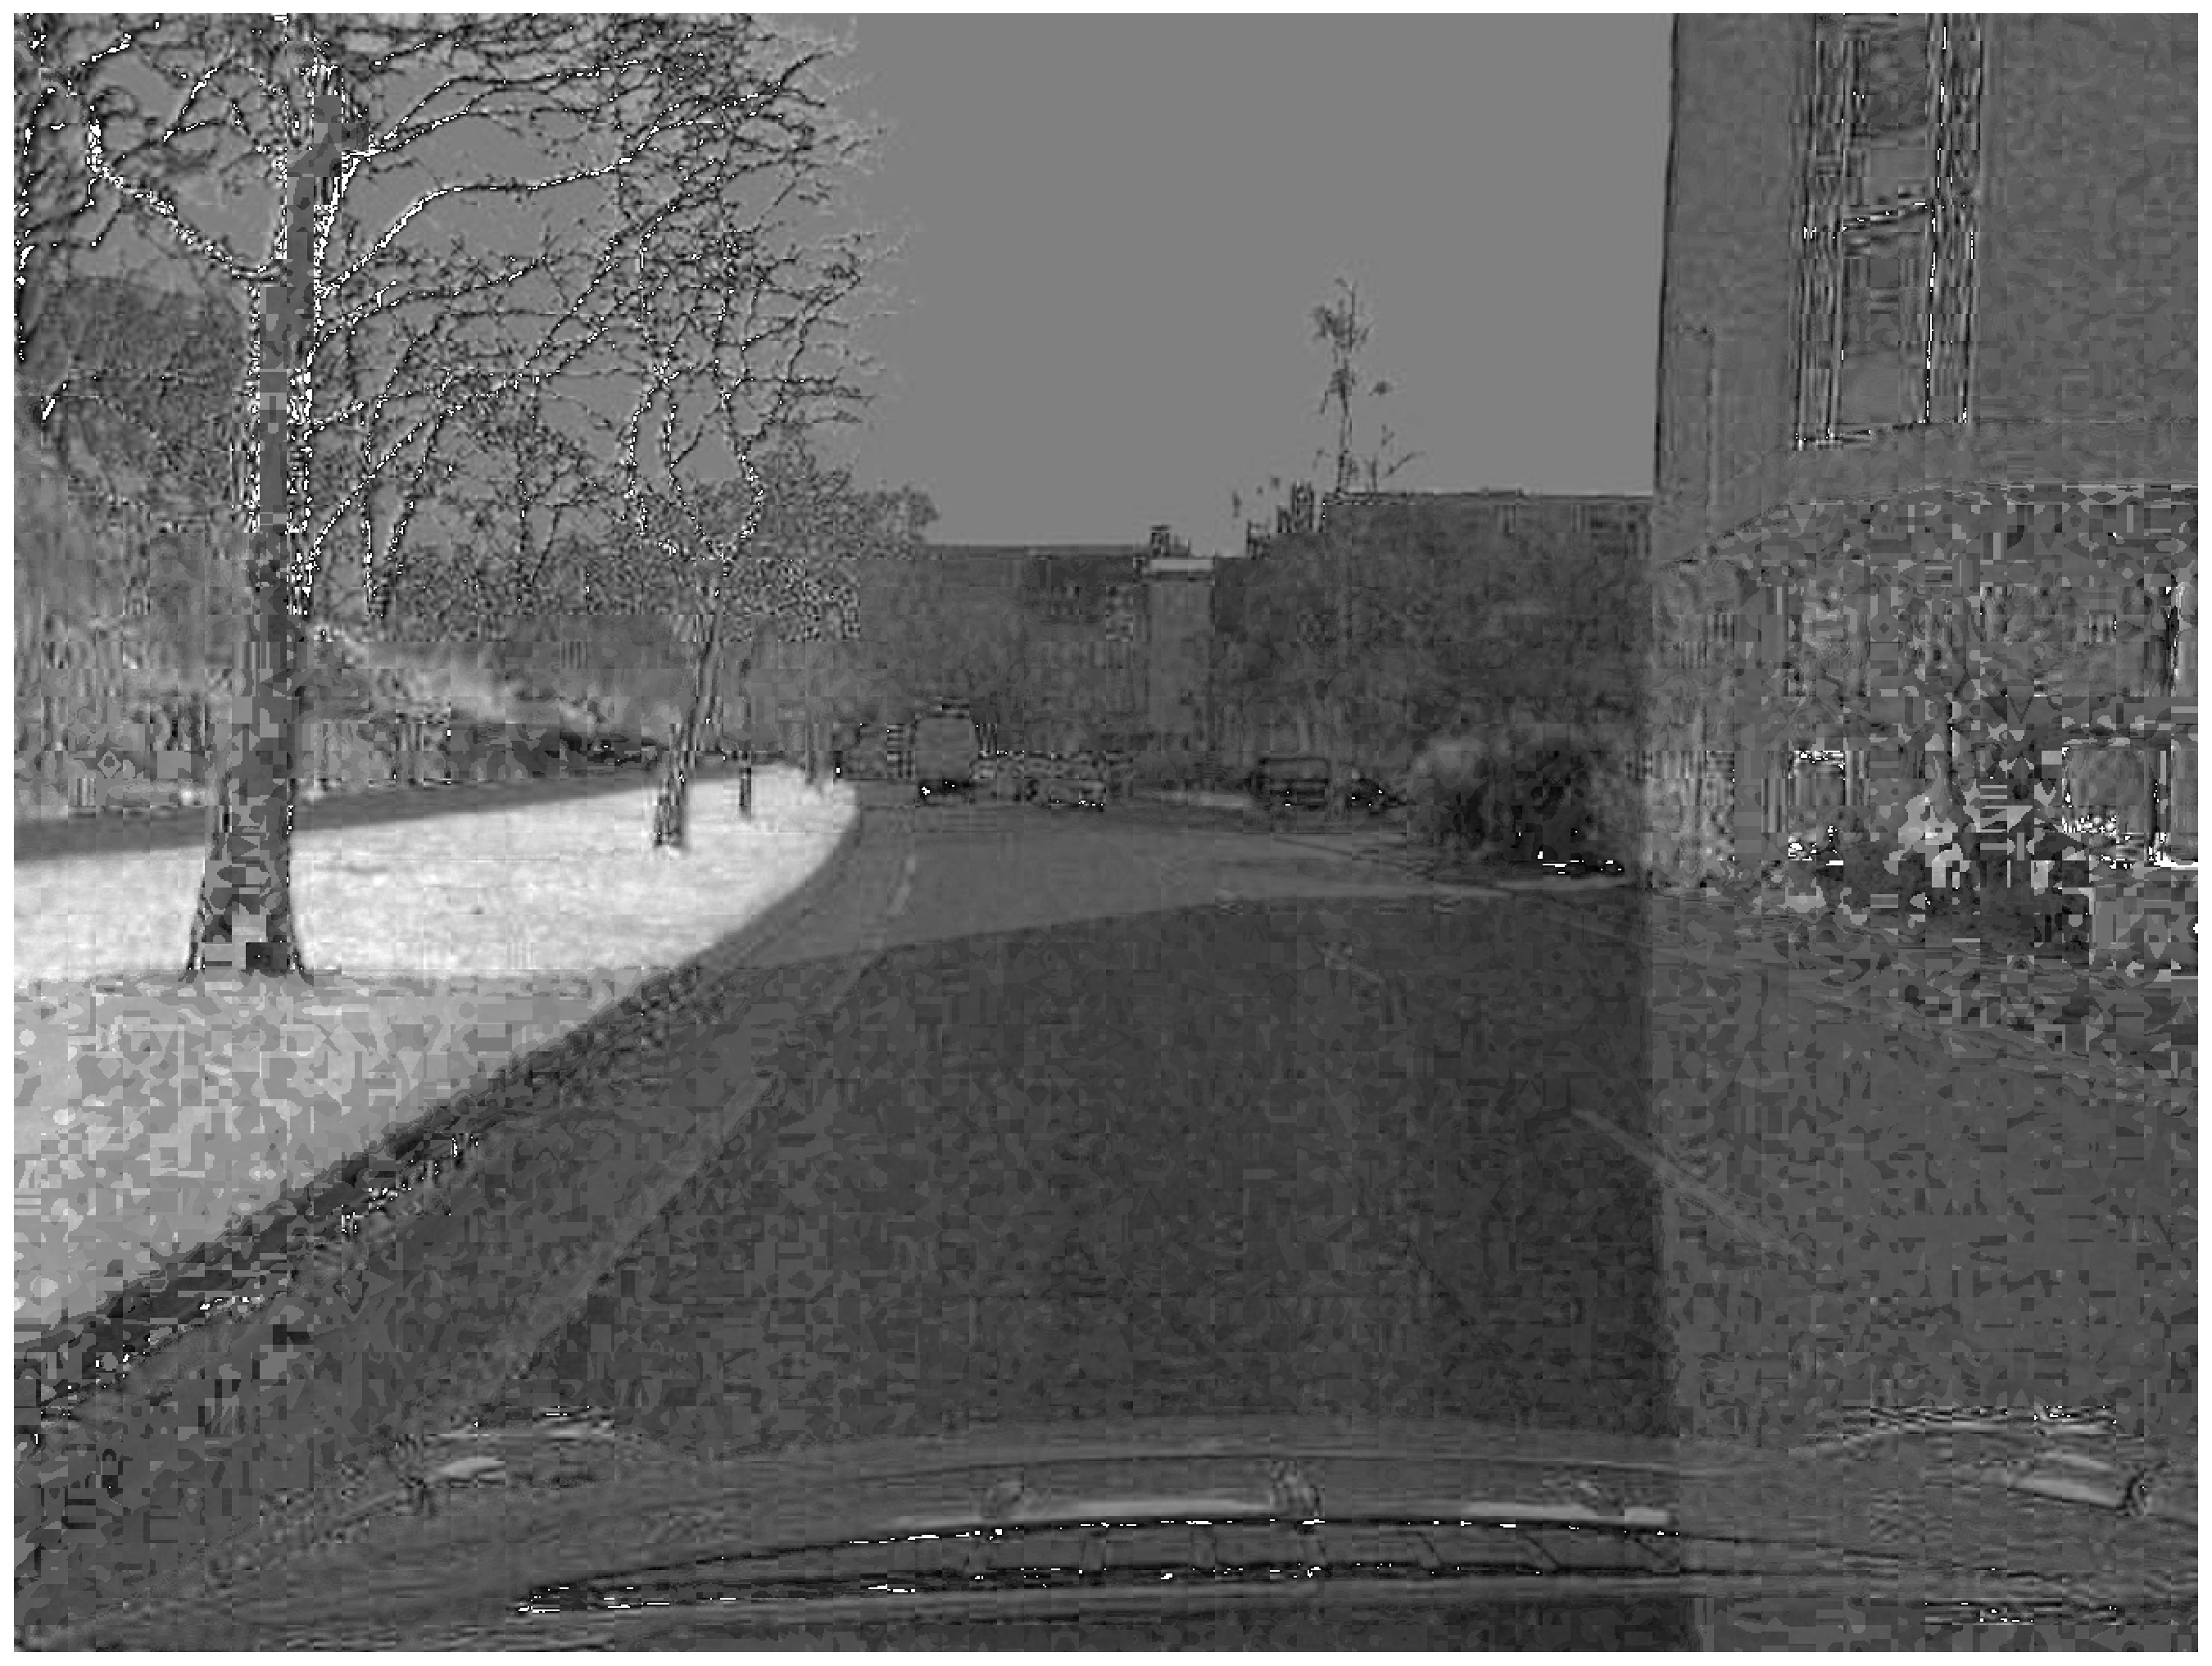
\includegraphics[width=4in]{Chapter4/robotcar/ill_inv2.eps}
			%\caption{fig2}
		\end{minipage}
	}
	\caption{Generated illumination variance images of example raw images in Oxford RobotCar Datasets.}
	\label{fig:discussrobotcarill}
\end{figure}

\begin{figure}[H]
	\centering
	\subfigure[Corresponding matched keypoint pairs of raw images Figure \ref{sfig:robotcarjulyraw} and \ref{sfig:robotcarfebraw}.]{
		\begin{minipage}[t]{\linewidth}
			\centering
			\includegraphics[width=5in]{Chapter4/robotcar/rawmatches.eps}
			\label{sfig:discussrobotcarrawmatch}
		\end{minipage}
	}
	\vfill
	\subfigure[Corresponding matched keypoint pairs of illumination variance images Figure \ref{sfig:robotcarjulyill} and \ref{sfig:robotcarfebill}.]{
		\begin{minipage}[t]{\linewidth}
			\centering
			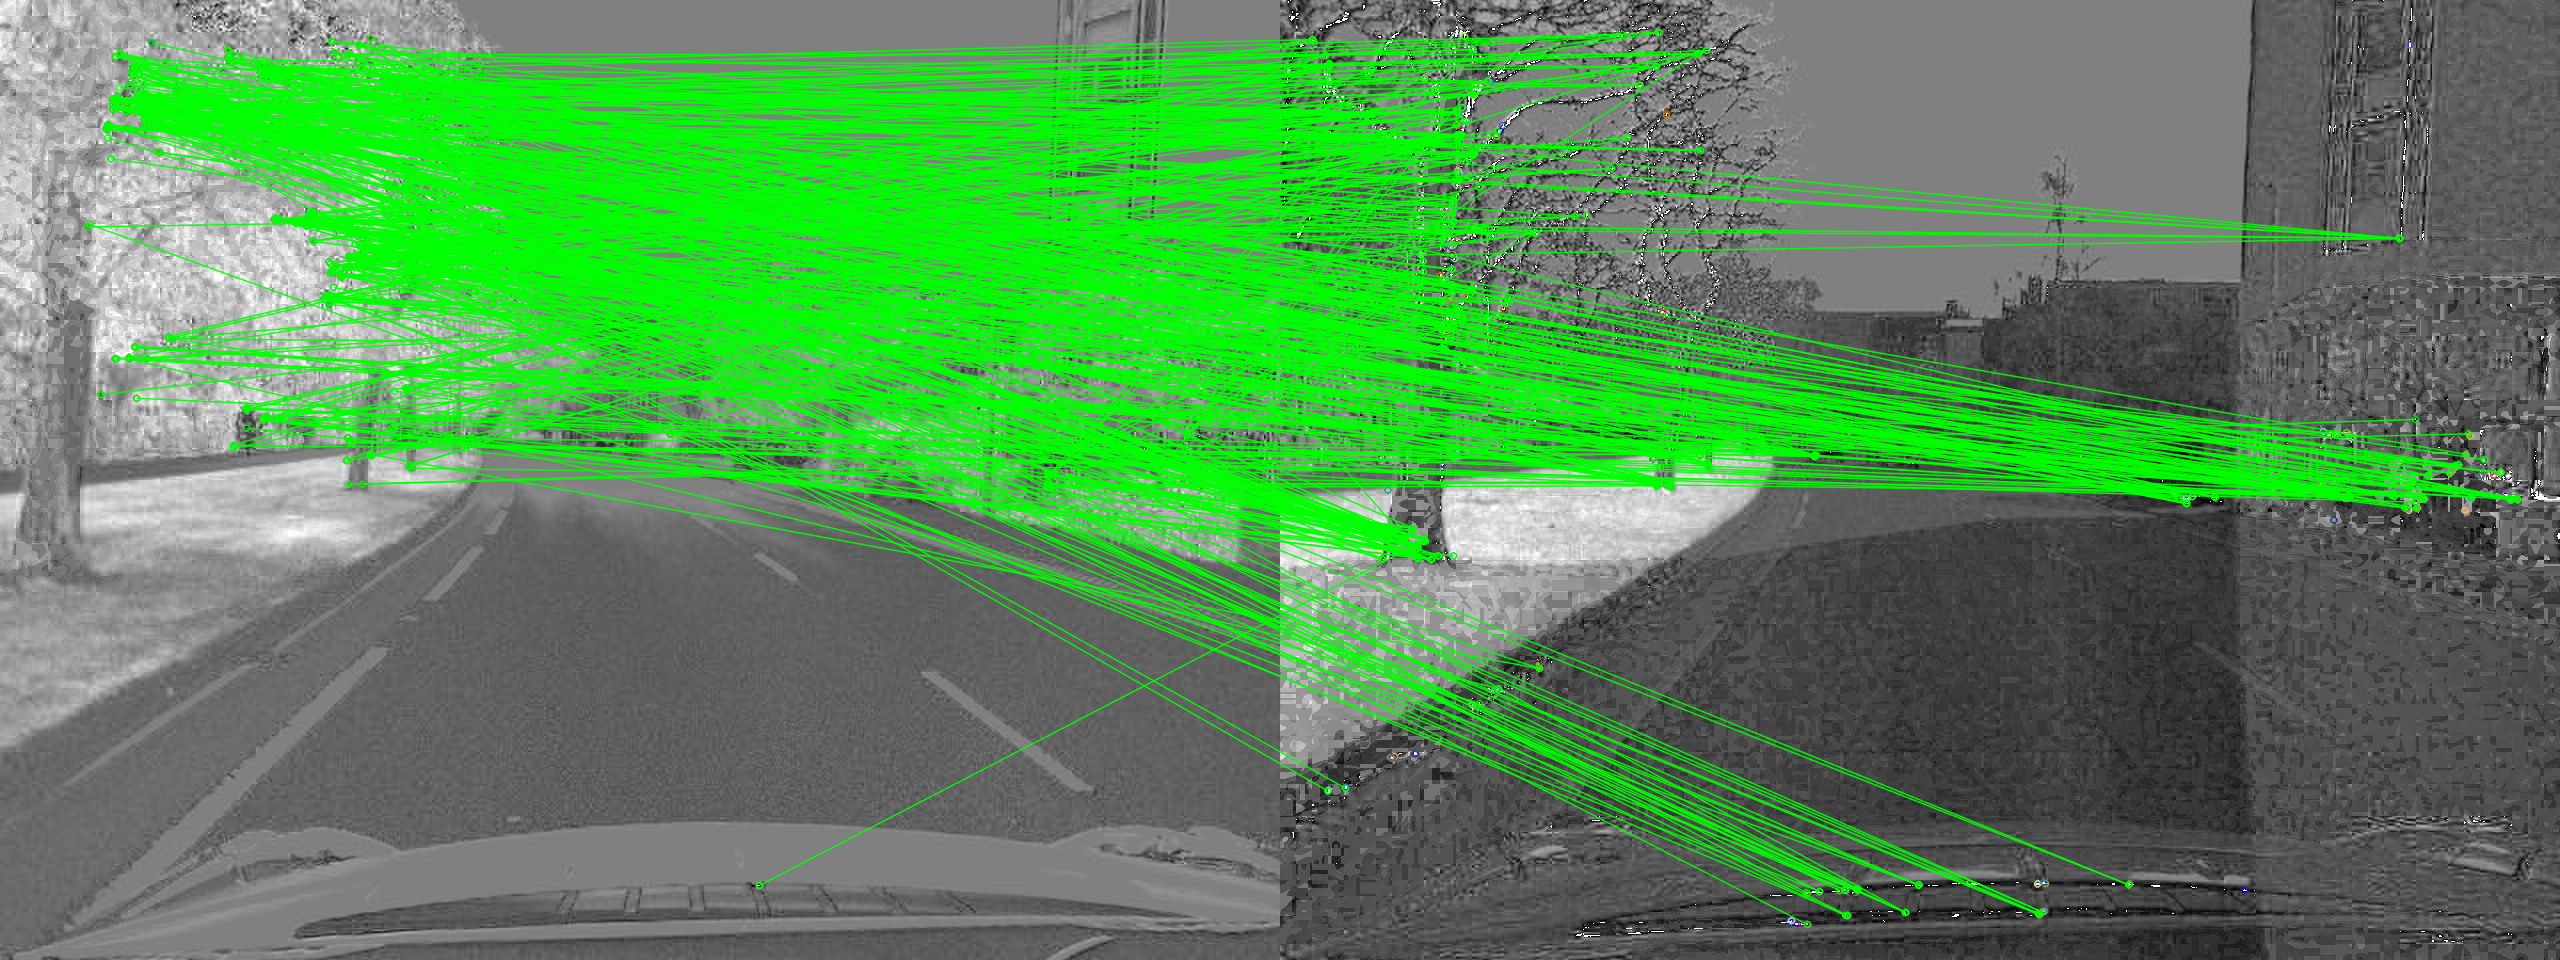
\includegraphics[width=5in]{Chapter4/robotcar/matches.eps}

			\label{sfig:discussrobotcarillmatch}
		\end{minipage}
	}
\caption{ORB Keypoint matching results of raw and illumination variance images in Oxford RobotCar Datasets.}
\label{fig:robotcarmatches}
\end{figure}

However, in both the original work \cite{maddern2014illumination} and the related implement in \cite{arroyo2014bidirectional,arroyo2014fast,arroyo2015towards,arroyo2016openable}, the application of this method only focus on localization, which means the main function is designed to detect loop closures in images taken in different illumination and seasons, but not suitable for mapping. In all above papers, evaluation results are given only by localization results.

A critical difference of localization and mapping tasks is high resolution images are not necessary in localization, while in mapping task they are. Cited by \cite{arroyo2014bidirectional}, \cite{milford2012visual}  explains that performing localization using a sequence of images rather than single image removes the requirement that the image matching scheme be able to reliably calculate a single global image match. However, without the functionality of calculating matches between single images, sequence-based image matching algorithms have significant drawbacks that cannot calculate the transformation between images.

And in the case of CORB-SLAM, the image matching algorithm combing ORB keypoint and Bag of Words, is able to calculate matching and transformation between individual images, but fit not well with illumination variance method.

%=== END OF CHAPTER FIVE ===
\newpage
